
\documentclass[letterpaper,hide notes,xcolor={table,svgnames},pdftex,10pt]{beamer}
\def\showexamples{t}

\usecolortheme{crane}
\setbeamertemplate{navigation symbols}{}

\usetheme{MyPittsburgh}
\usepackage{hyperref}
\usepackage{graphicx,xspace}
\usepackage[normalem]{ulem}
\usepackage{multicol}
\usepackage{amsmath,amssymb,amsthm,graphicx,xspace}
\newcommand\SF[1]{$\bigstar$\footnote{SF: #1}}

\usepackage[sfdefault,lf]{carlito}
\usepackage[T1]{fontenc}
\usepackage[scaled]{beramono}
\usepackage{tikzpagenodes}
\newcommand{\Rplus}{\protect\hspace{-.1em}\protect\raisebox{.35ex}{\small{\small\textbf{+}}}}
\newcommand{\Cpp}{\mbox{C\Rplus\Rplus}\xspace}

\newcounter{tmpnumSlide}
\newcounter{tmpnumNote}

\newcommand\mnote[1]{%
	\addtocounter{tmpnumSlide}{1}
	\ifdefined\showcues {~\tiny\fbox{\arabic{tmpnumSlide}}}\fi
	\note{\setlength{\parskip}{1ex}\addtocounter{tmpnumNote}{1}\textbf{\Large \arabic{tmpnumNote}:} {#1\par}}}

\newcommand\mmnote[1]{\note{\setlength{\parskip}{1ex}#1\par}}


\newcommand\mquestion[2]{{~\color{red}\fbox{?}}\note{\setlength{\parskip}{1ex}\par{\Large \textbf{?}} #1} \note{\setlength{\parskip}{1ex}\par{\Large \textbf{A}} #2\par}\ifdefined \presentationonly \pause \fi}

\newcommand\blackboard[1]{%
	\ifdefined   \showblackboard
		{#1}
	\else {\begin{center} \fbox{\colorbox{blue!30}{%
						\begin{minipage}{.95\linewidth}%
							\hspace{\stretch{1}} Some space intentionally left blank; done at the blackboard.%
						\end{minipage}}}\end{center}}%
	\fi%
}

\usepackage{listings}
\lstset{%
	keywordstyle=\bfseries,
	aboveskip=15pt,
	belowskip=15pt,
	captionpos=b,
	identifierstyle=\ttfamily,
	frame=lines,
	numbers=left, basicstyle=\scriptsize, numberstyle=\tiny, stepnumber=0, numbersep=2pt}

\usepackage{siunitx}
\newcommand\sius[1]{\num[group-separator = {,}]{#1}\si{\micro\second}}
\newcommand\sims[1]{\num[group-separator = {,}]{#1}\si{\milli\second}}
\newcommand\sins[1]{\num[group-separator = {,}]{#1}\si{\nano\second}}
\sisetup{group-separator = {,}, group-digits = true}

%% -------------------- tikz --------------------
\usepackage{tikz}
\usetikzlibrary{positioning}
\usetikzlibrary{arrows,backgrounds,automata,decorations.shapes,decorations.pathmorphing,decorations.markings,decorations.text}

\tikzstyle{place}=[circle,draw=blue!50,fill=blue!20,thick, inner sep=0pt,minimum size=6mm]
\tikzstyle{transition}=[rectangle,draw=black!50,fill=black!20,thick, inner sep=0pt,minimum size=4mm]

\tikzstyle{block}=[rectangle,draw=black, thick, inner sep=5pt]
\tikzstyle{bullet}=[circle,draw=black, fill=black, thin, inner sep=2pt]

\tikzstyle{pre}=[<-,shorten <=1pt,>=stealth',semithick]
\tikzstyle{post}=[->,shorten >=1pt,>=stealth',semithick]
\tikzstyle{bi}=[<->,shorten >=1pt,shorten <=1pt, >=stealth',semithick]

\tikzstyle{mut}=[-,>=stealth',semithick]

\tikzstyle{treereset}=[dashed,->, shorten >=1pt,>=stealth',thin]

\usepackage{ifmtarg}
\usepackage{xifthen}
\makeatletter
% new counter to now which frame it is within the sequence
\newcounter{multiframecounter}
% initialize buffer for previously used frame title
\gdef\lastframetitle{\textit{undefined}}
% new environment for a multi-frame
\newenvironment{multiframe}[1][]{%
	\ifthenelse{\isempty{#1}}{%
		% if no frame title was set via optional parameter,
		% only increase sequence counter by 1
		\addtocounter{multiframecounter}{1}%
	}{%
		% new frame title has been provided, thus
		% reset sequence counter to 1 and buffer frame title for later use
		\setcounter{multiframecounter}{1}%
		\gdef\lastframetitle{#1}%
	}%
	% start conventional frame environment and
	% automatically set frame title followed by sequence counter
	\begin{frame}%
		\frametitle{\lastframetitle~{\normalfont(\arabic{multiframecounter})}}%
		}{%
	\end{frame}%
}
\makeatother

\makeatletter
\newdimen\tu@tmpa%
\newdimen\ydiffl%
\newdimen\xdiffl%
\newcommand\ydiff[2]{%
	\coordinate (tmpnamea) at (#1);%
	\coordinate (tmpnameb) at (#2);%
	\pgfextracty{\tu@tmpa}{\pgfpointanchor{tmpnamea}{center}}%
	\pgfextracty{\ydiffl}{\pgfpointanchor{tmpnameb}{center}}%
	\advance\ydiffl by -\tu@tmpa%
}
\newcommand\xdiff[2]{%
	\coordinate (tmpnamea) at (#1);%
	\coordinate (tmpnameb) at (#2);%
	\pgfextractx{\tu@tmpa}{\pgfpointanchor{tmpnamea}{center}}%
	\pgfextractx{\xdiffl}{\pgfpointanchor{tmpnameb}{center}}%
	\advance\xdiffl by -\tu@tmpa%
}
\makeatother
\newcommand{\copyrightbox}[3][r]{%
	\begin{tikzpicture}%
		\node[inner sep=0pt,minimum size=2em](ciimage){#2};
		\usefont{OT1}{phv}{n}{n}\fontsize{4}{4}\selectfont
		\ydiff{ciimage.south}{ciimage.north}
		\xdiff{ciimage.west}{ciimage.east}
		\ifthenelse{\equal{#1}{r}}{%
			\node[inner sep=0pt,right=1ex of ciimage.south east,anchor=north west,rotate=90]%
			{\raggedleft\color{black!50}\parbox{\the\ydiffl}{\raggedright{}#3}};%
		}{%
			\ifthenelse{\equal{#1}{l}}{%
				\node[inner sep=0pt,right=1ex of ciimage.south west,anchor=south west,rotate=90]%
				{\raggedleft\color{black!50}\parbox{\the\ydiffl}{\raggedright{}#3}};%
			}{%
				\node[inner sep=0pt,below=1ex of ciimage.south west,anchor=north west]%
				{\raggedleft\color{black!50}\parbox{\the\xdiffl}{\raggedright{}#3}};%
			}
		}
	\end{tikzpicture}
}


%% --------------------

%\usepackage[excludeor]{everyhook}
%\PushPreHook{par}{\setbox0=\lastbox\llap{MUH}}\box0}

%\vspace*{\stretch{1}

%\setbox0=\lastbox \llap{\textbullet\enskip}\box0}

\setlength{\parskip}{\fill}

\newcommand\noskips{\setlength{\parskip}{1ex}}
\newcommand\doskips{\setlength{\parskip}{\fill}}

\newcommand\xx{\par\vspace*{\stretch{1}}\par}
\newcommand\xxs{\par\vspace*{2ex}\par}
\newcommand\tuple[1]{\langle #1 \rangle}
\newcommand\code[1]{{\sf \footnotesize #1}}
\newcommand\ex[1]{\uline{Example:} \ifdefined \presentationonly \pause \fi
	\ifdefined\showexamples#1\xspace\else{\uline{\hspace*{2cm}}}\fi}

\newcommand\ceil[1]{\lceil #1 \rceil}


\AtBeginSection[]
{
	\begin{frame}
		\frametitle{Outline}
		\tableofcontents[currentsection]
	\end{frame}
}



\pgfdeclarelayer{edgelayer}
\pgfdeclarelayer{nodelayer}
\pgfsetlayers{edgelayer,nodelayer,main}

\tikzstyle{none}=[inner sep=0pt]
\tikzstyle{rn}=[circle,fill=Red,draw=Black,line width=0.8 pt]
\tikzstyle{gn}=[circle,fill=Lime,draw=Black,line width=0.8 pt]
\tikzstyle{yn}=[circle,fill=Yellow,draw=Black,line width=0.8 pt]
\tikzstyle{empty}=[circle,fill=White,draw=Black]
\tikzstyle{bw} = [rectangle, draw, fill=blue!20,
text width=4em, text centered, rounded corners, minimum height=2em]

\newcommand{\CcNote}[1]{% longname
	This work is licensed under the \textit{Creative Commons #1 3.0 License}.%
}
\newcommand{\CcImageBy}[1]{%
	\includegraphics[scale=#1]{creative_commons/cc_by_30.pdf}%
}
\newcommand{\CcImageSa}[1]{%
	\includegraphics[scale=#1]{creative_commons/cc_sa_30.pdf}%
}
\newcommand{\CcImageNc}[1]{%
	\includegraphics[scale=#1]{creative_commons/cc_nc_30.pdf}%
}
\newcommand{\CcGroupBySa}[2]{% zoom, gap
	\CcImageBy{#1}\hspace*{#2}\CcImageNc{#1}\hspace*{#2}\CcImageSa{#1}%
}
\newcommand{\CcLongnameByNcSa}{Attribution-NonCommercial-ShareAlike}

\newenvironment{changemargin}[1]{% 
	\begin{list}{}{% 
		\setlength{\topsep}{0pt}% 
		\setlength{\leftmargin}{#1}% 
		\setlength{\rightmargin}{1em}
		\setlength{\listparindent}{\parindent}% 
		\setlength{\itemindent}{\parindent}% 
		      \setlength{\parsep}{\parskip}% 
		      }% 
		\item[]}{\end{list}}




\title{Lecture 23 --- Condition Variables, Monitors, Atomic Types }

\author{Jeff Zarnett \\ \small \texttt{jzarnett@uwaterloo.ca}}
\institute{Department of Electrical and Computer Engineering \\
  University of Waterloo}
\date{\today}


\begin{document}

\begin{frame}
  \titlepage

 \end{frame}


\begin{frame}
\frametitle{Condition Variables}

\begin{center}
	
\includegraphics[width=0.4\textwidth]{images/monday.png}
\end{center}

Condition variables are another way to achieve synchronization.

\end{frame}

\begin{frame}
\frametitle{Condition Variables}

How do we know if some condition has been fulfilled?

Signal on a semaphore?

Lock mutex, read variable(s), unlock mutex?

Or: a Condition Variable.

\end{frame}


\begin{frame}
\frametitle{Condition Variable}

We can think of condition variables as ``events'' that occur.

What differentiates it: broadcast!

We have the option, when an event occurs, to signal either one thread waiting for that event to occur, or to broadcast (signal) to all threads waiting for the event.

\end{frame}

\begin{frame}[fragile]
\frametitle{Condition Variable Syntax}

\begin{lstlisting}[language=C]
pthread_cond_init( pthread_cond_t *cv, pthread_condattr_t *attributes );
pthread_cond_wait( pthread_cond_t *cv, pthread_mutex_t *mutex );
pthread_cond_signal( pthread_cond_t *cv );
pthread_cond_broadcast( pthread_cond_t *cv );
pthread_cond_destroy( pthread_cond_t *cv );
\end{lstlisting}

As with other pthread functions we've seen there are create and destroy calls.

Signal is self-explanatory; but broadcast is new and wait looks weird!

\end{frame}


\begin{frame}
\frametitle{Wait, in Two Parts}

Condition variables are always used in conjunction with a mutex. 

\texttt{pthread\_cond\_wait} takes the condition variable and a mutex. 

This routine should be called only while the mutex is locked. 

It will automatically release the mutex while it waits for the condition!

When the condition is true, then the mutex will be automatically locked again so the thread may proceed.

Then, manually unlock when finished.

\end{frame}

\begin{frame}
\frametitle{HEY GUYS!!! GUESS WHAT!!!}
\begin{center}
	
\includegraphics[width=0.6\textwidth]{images/newsanchor.jpg}
\end{center}

\texttt{pthread\_cond\_broadcast} signals all threads waiting on that condition variable. 

It's this ``broadcast'' idea that makes the condition variable more interesting than the simple ``signalling'' pattern we covered much earlier on.

\end{frame}

\begin{frame}[fragile]
\frametitle{Condition Variable Example}

\begin{lstlisting}[language=C]
#include <pthread.h>
#include <stdio.h>
#include <stdlib.h>

#define NUM_THREADS  3
#define COUNT_LIMIT 12

int count = 0;
pthread_mutex_t count_mutex;
pthread_cond_t count_threshold_cv;

void* inc_count( void* arg ) {
  for (int i = 0; i < 10; i++ ) {
    pthread_mutex_lock( &count_mutex );
    count++;
    if ( count == COUNT_LIMIT ) {
      printf( "Condition Fulfilled!\n" );
      pthread_cond_signal( &count_threshold_cv );
      printf( "Sent signal.\n" );
    }
    pthread_mutex_unlock( &count_mutex );
  }
  pthread_exit( NULL );
}
\end{lstlisting}
\end{frame}

\begin{frame}[fragile]
\frametitle{Condition Variable Example}

\begin{lstlisting}[language=C]
void* watch_count( void *arg ) {
  pthread_mutex_lock( &count_mutex );  
  if ( count < COUNT_LIMIT ) {
    pthread_cond_wait( &count_threshold_cv, &count_mutex );
    printf( "Watcher has woken up.\n" );
    /* Do something useful here now that condition is fulfilled. */
  }
  pthread_mutex_unlock( &count_mutex );
  pthread_exit( NULL );
}
\end{lstlisting}
\end{frame}

\begin{frame}[fragile]
\frametitle{Condition Variable Example}
\begin{lstlisting}[language=C]
int main( int argc, char **argv ) {
  pthread_t threads[3];

  pthread_mutex_init( &count_mutex, NULL );
  pthread_cond_init ( &count_threshold_cv, NULL );

  pthread_create( &threads[0], NULL, watch_count, NULL );
  pthread_create( &threads[1], NULL, inc_count, NULL );
  pthread_create( &threads[2], NULL, inc_count, NULL );

  for ( int i = 0; i < NUM_THREADS; i++ ) {
    pthread_join(threads[i], NULL);
  }
  
  pthread_mutex_destroy( &count_mutex );
  pthread_cond_destroy( &count_threshold_cv );
  pthread_exit( NULL );
}
\end{lstlisting}
\end{frame}


\begin{frame}
\frametitle{Anybody Listening?}

If a thread signals a condition variable that an event has occurred, but no thread is waiting for that event, the event is ``lost''. 

This is sometimes called the ``lost wakeup problem'', because threads don't get woken up if they weren't waiting for this. 

That's usually an error, but it might be acceptable.

\end{frame}

\begin{frame}
\frametitle{Can We Apply This To What We Know?}

The condition variable with broadcast can be used to replace some of the synchronization constructs we've seen already. 

What patterns could be replaced?

\end{frame}

\begin{frame}[fragile]
\frametitle{Broadcast Barrier}

Consider the barrier pattern from earlier. 

There are $n$ threads and we wait for the last one to arrive.
{\scriptsize
\begin{multicols}{2}
  \begin{verbatim}
	1. wait( mutex )
	2. count++
	3. if count == n
	4.     post( barrier )
	5. end if
	6. post( mutex )
	7. wait( barrier )
	8. post( barrier )
  \end{verbatim}
\columnbreak
  \begin{verbatim}
	1. wait( mutex )
	2. count++
	3. if count < n
	4.     cond_wait( barrier, mutex )
	5. else 
	6.     cond_broadcast( barrier )
	7. end if
	8. post( mutex )
  \end{verbatim}
\end{multicols}
}

The \texttt{wait} takes place before the post on \texttt{mutex}. That looks strange, doesn't it?

\end{frame}


\begin{frame}
\frametitle{Spidey Sense Tingling?}


We give up the mutex \texttt{lock} when we wait on the condition variable.

The fact that we don't get to the unlock statement first does not cause a problem. 

So we are alright. 

The last thread doesn't wait on the condition at all because there's no need to!

It knows that it is last and there's nothing to wait for so it should proceed.

\end{frame}

\begin{frame}[fragile]
\frametitle{Barrier Pattern Code Example}
\begin{lstlisting}[language=C]
int count;
pthread_mutex_t lock;
pthread_cond_t cv; 

void barrier( ) {
  pthread_mutex_lock( &lock );
  count++;
  if ( count < NUM_THREADS ) {
    pthread_cond_wait( &cv, &lock );
  } else {
    pthread_cond_broadcast( &cv );
  }
  pthread_mutex_unlock( &lock );
}
\end{lstlisting}

Will this work?

\end{frame}


\begin{frame}
\frametitle{Monitors}
\begin{center}
	
\includegraphics[width=0.5\textwidth]{images/monitor.jpg}
\end{center}

Uh... wait... this isn't the right kind.

\end{frame}

\begin{frame}
\frametitle{What's a Monitor?}

A condition variable can be used to create a \alert{monitor}, a higher level synchronization construct. 

This is a bit like in OOP the idea of a class.

When we use a monitor we are packaging up the shared data and operations on that data.

Eliminate the need to write synchronization code ourselves.

\end{frame}


\begin{frame}[fragile]
\frametitle{Did We Forget Something?}

\begin{lstlisting}[language=C]
void foo( ) {
  pthread_mutex_lock( &l );
  /* Read some data */
  if ( condition ) {
    printf( "Cannot continue due to reasons...\n" );
    return;
  }
  /* More stuff */
   
  pthread_mutex_unlock( &l );
}
\end{lstlisting}

\end{frame}


\begin{frame}
\frametitle{Control Flow Problems}

There is control flow that could lead to exiting this function \texttt{foo} without unlocking the mutex \texttt{l}.

It looks super obvious in this case, but in real life it's harder to see!

\end{frame}

\begin{frame}[fragile]
\frametitle{Java Anyone?}

The idea of monitors should be familiar to you if you have used Java synchronization constructs, notably the \texttt{synchronized} keyword. 

In Java we can declare a method to be \texttt{synchronized}.

There is a lock created around that method. Locking and unlocking is handled automatically.

\begin{lstlisting}[language=Java]
public synchronized void doSomething() {
    // Synchronized area
}
\end{lstlisting}

\end{frame}

\begin{frame}[fragile]
\frametitle{Synchronized Blocks}

in Java one can also define a block as synchronized:

\begin{lstlisting}[language=Java]
public void exampleMethod() {
    synchronized( object ) { // Lock must be acquired to enter this block
           // Critical section 
    } // Lock is automatically released.
}
\end{lstlisting}

This sort of ``automatic'' locking and releasing is intended to simplify the process of writing multithreaded code.

\end{frame}

\begin{frame}
\frametitle{This isn't an endorsement of Java...}

Monitors don't have to be written in Java (or similar).

They do frequently appear in Object-Oriented languages because the concepts are familiar enough.


\end{frame}

\begin{frame}
\frametitle{Atomic Types}
\begin{center}
	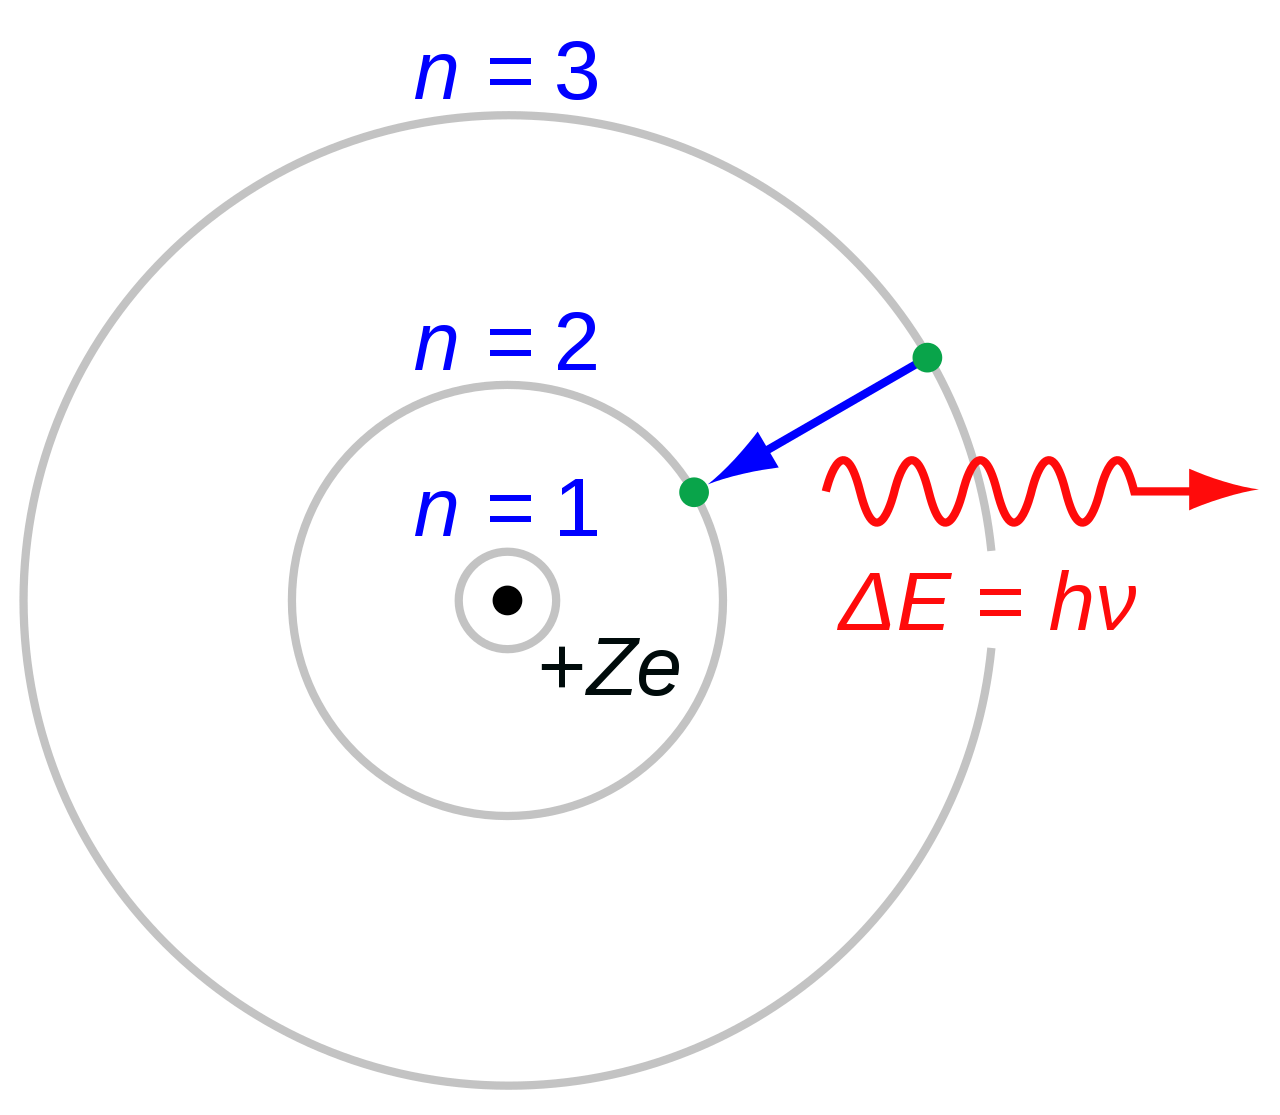
\includegraphics[width=0.5\textwidth]{images/bohrmodel.png}
\end{center}
\hfill Image Credit: Wikipedia user JabberWok

A testament to how good humans are at blowing things up...

\end{frame}



\begin{frame}[fragile]
\frametitle{Atomic Types}

Frequently we have a code pattern that looks something like this:

\begin{lstlisting}[language=C]
pthread_mutex_lock( lock );
shared_var++;
pthread_mutex_unlock( lock );
\end{lstlisting}

It seems like a lot of work to lock and unlock the mutex, no?

Thinking back to the ``test and set'' type of instruction from earlier, wouldn't it be nice if we could do that sort of thing for something like incrementing a variable?

\end{frame}

\begin{frame}
\frametitle{Hey Kernel, Could You Please...}

The Linux kernel provides operations that are guaranteed to execute atomically, to avoid simple race conditions. 

In a uniprocessor system, the CPU cannot be interrupted until the operation is finished. 

In a multiprocessor system, the variable is locked until the operation is finished.

 There are two types of atomic operations: those that operate on integers and those that operate on a single bit in a bitmap.

\end{frame}

\begin{frame}
\frametitle{Prevent Confusion}

Rather than just using an integer for atomic integer operations, there is a defined type \texttt{atomic\_t}.

 This prevents programming errors and hides architecture-specific implementation details.

\end{frame}


\begin{frame}
\frametitle{Operation Table}

{\scriptsize
\begin{center}
\begin{tabular}{l|l}
	\textbf{Function} & \textbf{Description}\\\hline

	\texttt{atomic\_t ATOMIC\_INIT( int i )} & At declaration, initialize an \texttt{atomic\_t} to \texttt{i}\\\hline

\texttt{int atomic\_read( atomic\_t *v )} &  Read the integer value of \texttt{v}\\\hline

\texttt{void atomic\_set( atomic\_t *v, int i )} & Set \texttt{v} equal to \texttt{i}\\\hline

\texttt{void atomic\_add( int i, atomic\_t *v )} & Add \texttt{i} to \texttt{v}\\\hline

\texttt{void atomic\_sub( int i, atomic\_t *v )} & Subtract \texttt{i} from \texttt{v}\\\hline

\texttt{void atomic\_inc( atomic\_t *v )} & Add 1 to \texttt{v}\\\hline

\texttt{void atomic\_dec( atomic\_t *v )} & Subtract 1 from \texttt{v}\\\hline

\texttt{int atomic\_sub\_and\_test( int i, atomic\_t *v )} & Subtract \texttt{i} from \texttt{v}; return true if 0; otherwise false\\\hline

\texttt{int atomic\_add\_negative( int i, atomic\_t *v )} & Add \texttt{i} to \texttt{v}; return true if negative; otherwise false\\\hline

\texttt{int atomic\_dec\_and\_test( atomic\_t *v )} & Decrement \texttt{v} by 1; return true if 0; otherwise false\\\hline

\texttt{int atomic\_inc\_and\_test( atomic\_t *v )} & Increment \texttt{v} by 1; return true if 0; otherwise false\\ \hline\hline

\texttt{void set\_bit( int n, void *addr )} &  Set the $n^{th}$ bit starting from \texttt{addr}\\\hline

\texttt{void clear\_bit( int n, void *addr )} &  Clear the $n^{th}$ bit starting from \texttt{addr}\\\hline

\texttt{void change\_bit( int n, void *addr )} &  Flip the value of the $n^{th}$ bit starting from \texttt{addr}\\\hline

\texttt{int test\_and\_set\_bit( int n, void *addr )} &  Set $n^{th}$ bit starting from \texttt{addr}; return previous value\\\hline

\texttt{int test\_and\_clear\_bit( int n, void *addr )} &  Clear $n^{th}$ bit starting from \texttt{addr}; return previous value\\\hline

\texttt{int test\_and\_change\_bit( int n, void *addr )} &  Flip $n^{th}$ bit starting from \texttt{addr}; return previous value\\\hline

\texttt{int test\_bit( int n, void *addr )} &  Return value of $n^{th}$ bit starting from \texttt{addr}\\\hline

\end{tabular}
\end{center}
}

These are Linux-specific and not portable (necessarily).

\end{frame}


\begin{frame}[fragile]
\frametitle{Use Tool Appropriately}

\begin{lstlisting}[language=C]
struct point {
  atomic_t x;
  atomic_t y;
};
atomic_set( p1->x, 0 );
atomic_set( p1->y, 0 );

/* Somewhere else in the program */
atomic_set( p1->x, 25 );
atomic_set( p1->y, 30 );
\end{lstlisting}

Does this work?

\end{frame}


\begin{frame}
\frametitle{Use Tool Appropriately}

Although the set of each of \texttt{x} and \texttt{y} is atomic, the operation as a whole is not.

Although the set of each of \texttt{x} and \texttt{y} is atomic, the operation as a whole is not.

\end{frame}


\begin{frame}
\frametitle{You Spin Me Right Round...}

Another common technique for protecting a critical section in Linux is the \textit{spinlock}.

This is a handy way to implement constant checking to acquire a lock. 

Unlike semaphores where the process is blocked if it fails to acquire the lock, a thread will constantly try to acquire the lock. 

When would we want this behaviour?

\end{frame}


\begin{frame}
\frametitle{When It's Worth It!}

It would be better to let another thread execute.

Except when the amount of time waiting on the lock might be small.

Specifically, less than it would take to block the process, switch to another, and unblock it when the value changes.


\end{frame}

\begin{frame}[fragile]
\frametitle{Spinlock}

\begin{lstlisting}[language=C]
spin_lock( &lock )
    /* Critical Section */
spin_unlock( &lock )
\end{lstlisting}


In addition to the regular spinlock, there are \textit{reader-writer-spinlocks}.

Like the readers-writers problem discussed earlier, the goal is to allow multiple readers but give exclusive access to a writer. 

\begin{center}
\begin{tabular}{l|l|l}
	\textbf{Counter} & \textbf{Flag} & \textbf{Interpretation}\\\hline
	0 & 1 & The spinlock is released and available. \\
	0 & 0 & The spinlock has been acquired for writing.\\
	$n$ ($n > 0$) & 0 & The spin lock has been acquired for reading by $n$ threads.\\
	$n$ ($n > 0$) & 1 & Invalid state.\\
\end{tabular}
\end{center}


\end{frame}



\end{document}

